\documentclass{standalone}
\usepackage{amsmath}
\usepackage{tikz}
\begin{document}
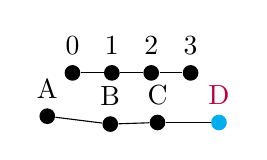
\begin{tikzpicture}
\node[fill=black, circle, inner sep=2pt, label=above:{\textcolor{black}{$\text{0}$} }] (Graph with 4 nodes and 3 edgesN0) at (3.7,-0.2) {};
\node[fill=black, circle, inner sep=2pt, label=above:{\textcolor{black}{$\text{1}$} }] (Graph with 4 nodes and 3 edgesN1) at (4.2,-0.2) {};
\node[fill=black, circle, inner sep=2pt, label=above:{\textcolor{black}{$\text{2}$} }] (Graph with 4 nodes and 3 edgesN2) at (4.7,-0.2) {};
\node[fill=black, circle, inner sep=2pt, label=above:{\textcolor{black}{$\text{3}$} }] (Graph with 4 nodes and 3 edgesN3) at (5.2,-0.2) {};
\draw[draw=black, shorten >=3pt, shorten <=3pt] (3.7,-0.2) -- (4.2,-0.2);
\draw[draw=black, shorten >=3pt, shorten <=3pt] (4.2,-0.2) -- (4.7,-0.2);
\draw[draw=black, shorten >=3pt, shorten <=3pt] (4.7,-0.2) -- (5.2,-0.2);
\node[fill=black, circle, inner sep=2pt, label=above:{\textcolor{black}{$\text{A}$} }] (Graph with 4 nodes and 3 edgesNA) at (3.38,-0.75) {};
\node[fill=black, circle, inner sep=2pt, label=above:{\textcolor{black}{$\text{B}$} }] (Graph with 4 nodes and 3 edgesNB) at (4.18,-0.85) {};
\node[fill=black, circle, inner sep=2pt, label=above:{\textcolor{black}{$\text{C}$} }] (Graph with 4 nodes and 3 edgesNC) at (4.78,-0.83) {};
\node[fill=cyan, circle, inner sep=2pt, label=above:{\textcolor{purple}{$\text{D}$} }] (Graph with 4 nodes and 3 edgesND) at (5.56,-0.83) {};
\draw[draw=black, shorten >=3pt, shorten <=3pt] (3.38,-0.75) -- (4.18,-0.85);
\draw[draw=black, shorten >=3pt, shorten <=3pt] (4.18,-0.85) -- (4.78,-0.83);
\draw[draw=black, shorten >=3pt, shorten <=3pt] (4.78,-0.83) -- (5.56,-0.83);
\end{tikzpicture}
\end{document}
